\documentclass{article}

\usepackage[english]{babel}
\usepackage[letterpaper,top=2cm,bottom=2cm,left=3cm,right=3cm]{geometry}
\usepackage{amsmath,amssymb}
\usepackage{graphicx}
\usepackage{float}
\usepackage{subcaption}
\usepackage{listings}
\lstset{basicstyle=\ttfamily\small,breaklines=true,frame=single,language=Python}

\title{\textbf{Humanoid Sensors and Actuators}\\
        Tutorial 5 – Acoustic Sensors and Signal Processing\\[4pt]
        Full Report}
\author{Binkun Huang \and Luca Hu \and Liangyu Chen}
\date{Summer Semester 2025}

\begin{document}
\maketitle



%--------------------------------------------------------------------
\section{Sound Source Localisation}

\subsection*{R.1.1 (3 pts)}
\emph{Find the expression to determine the azimuth angle of a sound source for a system with two microphones. Derive the equations shown in the slides of Lecture 3 step by step.}



\subsection*{R.1.2 (3 pts)}
\emph{Find the expression to determine the velocity of a target from the pulse duration difference of a radar sensor. Derive the equations shown in the slides of Lecture 3 step by step.}

\subsection*{R.1.3 (1 pt)}
\emph{How can we measure the distance to a target?}


\subsection*{R.1.4 (1 pt)}
\emph{How can we measure the speed of a moving target?}


%--------------------------------------------------------------------
\section{Fast Fourier Transform}

\subsection*{Task results (T.2.1 – T.2.4)}
\begin{figure}[H]
\centering
\begin{subfigure}{0.45\linewidth}
  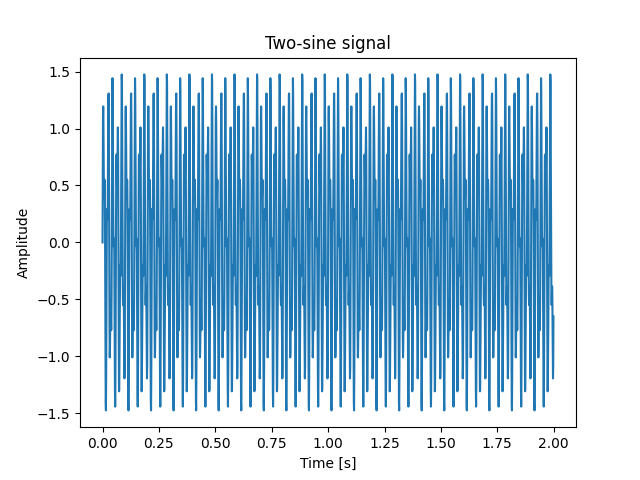
\includegraphics[width=\linewidth]{results/figures/task2_1_sum_two_sine_waves.png}
  \caption{Two‑sine signal (T.2.1)}
\end{subfigure}\hfill
\begin{subfigure}{0.45\linewidth}
  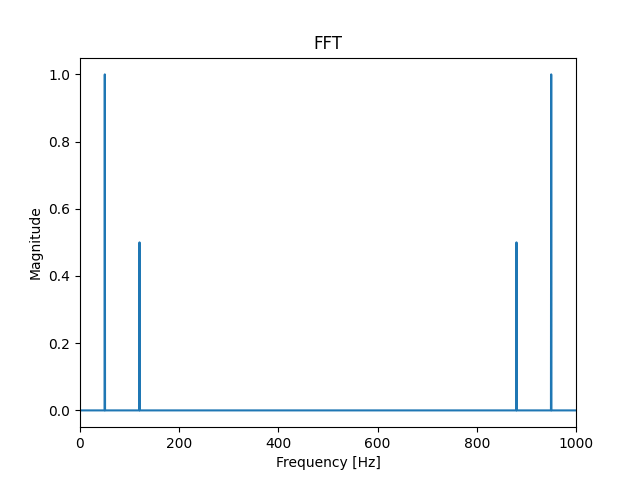
\includegraphics[width=\linewidth]{results/figures/task2_2_normalized_spectrum.png}
  \caption{FFT of clean signal (T.2.2)}
\end{subfigure}

\medskip
\begin{subfigure}{0.45\linewidth}
  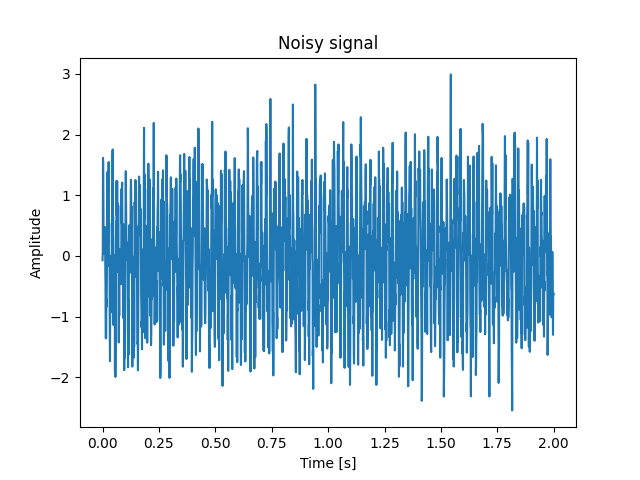
\includegraphics[width=\linewidth]{results/figures/task2_3_noisy_signal.png}
  \caption{Signal with Gaussian noise (T.2.3)}
\end{subfigure}\hfill
\begin{subfigure}{0.45\linewidth}
  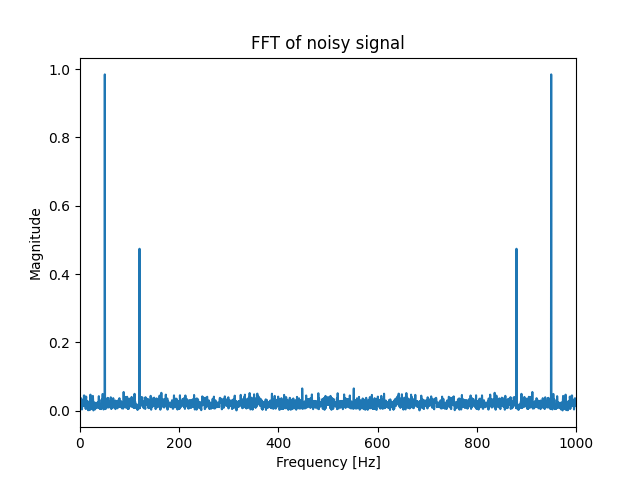
\includegraphics[width=\linewidth]{results/figures/task2_4_noisy_spectrum.png}
  \caption{FFT of noisy signal (T.2.4)}
\end{subfigure}
\end{figure}

\subsection*{R.2.1 (2 pts)}
\emph{Is it possible to implement FFT to an online data streaming? Why?}

FFT cannot directly process samples one-by-one in real-time. It needs data segments of fixed length (usually a power of two). Thus, FFT can only be applied to streaming data by dividing it into windows or segments.

\subsection*{R.2.2 (2 pts)}
\emph{How can you use FFT in signal processing?}

FFT transforms signals from the time domain into the frequency domain. This is useful for analyzing frequency components, identifying dominant frequencies, filtering noise, and extracting spectral features.

\subsection*{R.2.3 (2 pts)}
\emph{Deliver the code used to generate the signals and plots?}

The code used is located in \texttt{scripts/task2\_fft.py}, which calls utility functions from \texttt{src/signal\_generation.py} and \texttt{src/fft\_utils.py}. A simplified excerpt is shown below:

\begin{verbatim}
from src.signal_generation import sum_sine_waves, add_noise
from src.fft_utils import compute_fft
import matplotlib.pyplot as plt

fs = 1000
duration = 2.0
components = [(50, 1.0), (120, 0.5)]
t, signal = sum_sine_waves(components, fs, duration)

freqs, mag = compute_fft(signal, fs, full_range=True)

noisy_signal = add_noise(signal, 0.5)
freqs_n, mag_n = compute_fft(noisy_signal, fs, full_range=True)
...
\end{verbatim}



%--------------------------------------------------------------------
\section{ Audio Correlation}

\subsection*{Task results (T.3.1 – T.3.8)}
\begin{figure}[H]
\centering
\begin{subfigure}{0.45\linewidth}
  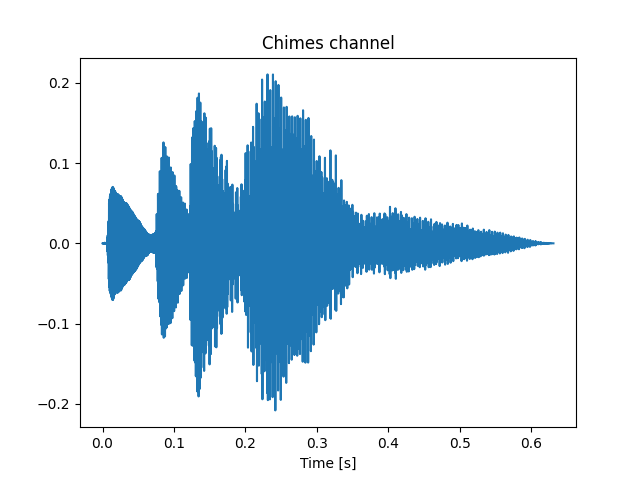
\includegraphics[width=\linewidth]{results/figures/task3_1_original_signal.png}
  \caption{Isolated channel (T.3.1)}
\end{subfigure}\hfill
\begin{subfigure}{0.45\linewidth}
  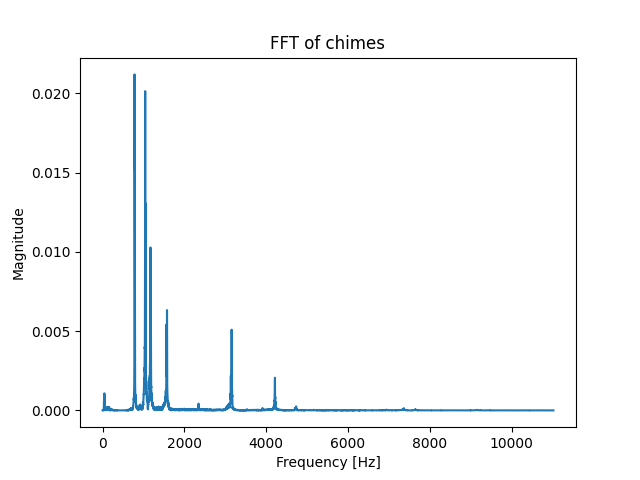
\includegraphics[width=\linewidth]{results/figures/task3_2_chimes_fft.png}
  \caption{FFT (T.3.2)}
\end{subfigure}

\medskip
\begin{subfigure}{0.45\linewidth}
  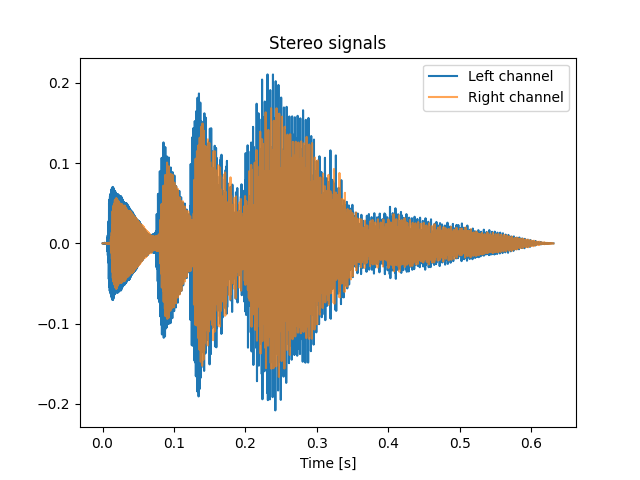
\includegraphics[width=\linewidth]{results/figures/task3_4_signals_with_scaling_and_delay.png}
  \caption{Stereo pair (T.3.3/3.4)}
\end{subfigure}\hfill
\begin{subfigure}{0.45\linewidth}
  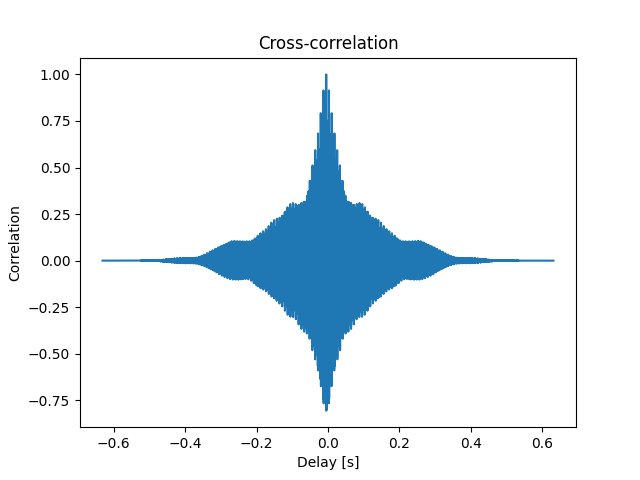
\includegraphics[width=\linewidth]{results/figures/task3_6_cross_correlation.png}
  \caption{Cross‑correlation (T.3.6)}
\end{subfigure}

\medskip
\begin{subfigure}{0.45\linewidth}
  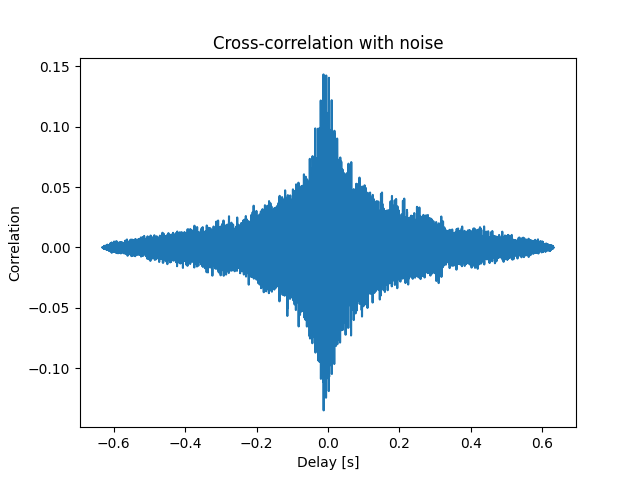
\includegraphics[width=\linewidth]{results/figures/task3_8_cross_correlations.png}
  \caption{Cross‑correlation with noise (T.3.8)}
\end{subfigure}
\end{figure}

\subsection*{R.3.1 (2 pts)}
\emph{Is it possible to implement the cross-correlation to an online data streaming? Why?}

No. Classical cross-correlation needs the complete sequences to evaluate every possible lag, so it is not a true sample-by-sample real-time algorithm. In streaming, the future samples are still unknown; therefore the full correlation map cannot be produced without buffering a window of past \emph{and} future data.

\subsection*{R.3.2 (2 pts)}
\emph{If you answered “no” to R.3.1, how would you work around to use it to identify the interaural time delay?}

Use a short sliding window whose length only covers plausible interaural delays (e.g.\ $\pm1$ ms). Update the window each time new samples arrive and compute the correlation (or GCC-PHAT) inside that window. The delay corresponding to the peak in each window gives an online estimate of the interaural time delay with acceptable latency.

\subsection*{R.3.3 (4 pts)}
\emph{Deliver the code to generate the signals and the plots (T.3.1 – T.3.8).}

The implementation is in \texttt{scripts/task3\_correlation.py}; it relies on helper functions in \texttt{src/correlation\_utils.py}, \texttt{src/fft\_utils.py} and \texttt{src/signal\_generation.py}. Key lines are:

\begin{verbatim}
data, fs = sf.read("data/chimes.wav")
mono = data[:, 0]              # T.3.1
freqs, mag = compute_fft(mono, fs)  # T.3.2

delay_samples = int(0.005 * fs)
left  = mono
right = np.roll(mono, delay_samples) * 0.8  # T.3.3

lags,  corr  = cross_correlation(left, right)       # T.3.6
left_n  = add_noise(left, 0.1)
right_n = add_noise(right, 0.1)
lags_n, corr_n = cross_correlation(left_n, right_n) # T.3.8
...
\end{verbatim}


%--------------------------------------------------------------------
\section{Signal Filtering}

\subsection*{Task results (T.4.1 – T.4.12)}
\begin{figure}[H]
\centering
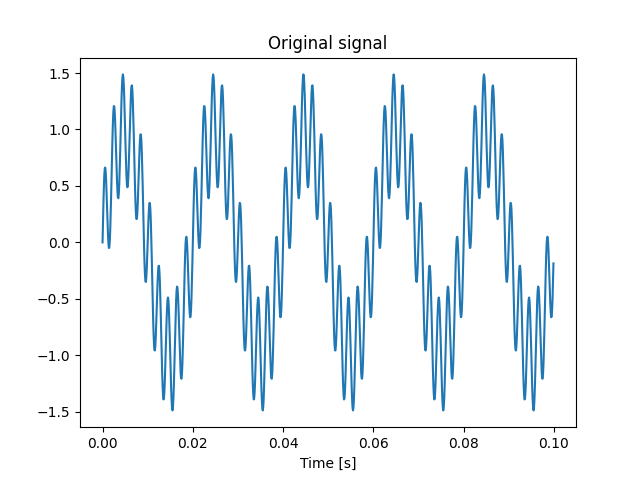
\includegraphics[width=0.45\linewidth]{results/figures/task4_2_sum_of_two_sine_waves.png}
\hfill
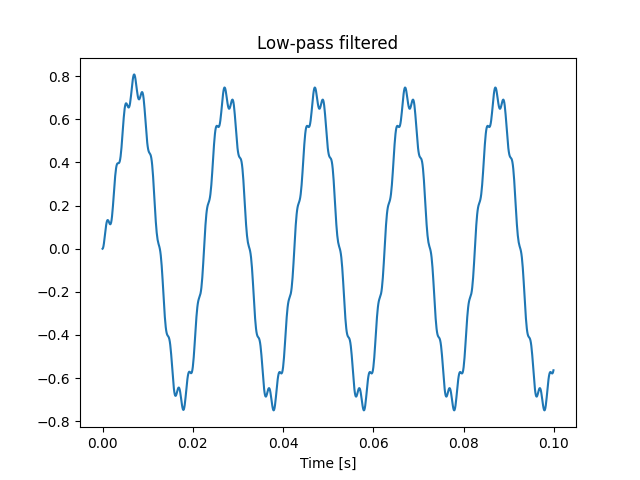
\includegraphics[width=0.45\linewidth]{results/figures/task4_5_lowpass_filtered.png}

\medskip
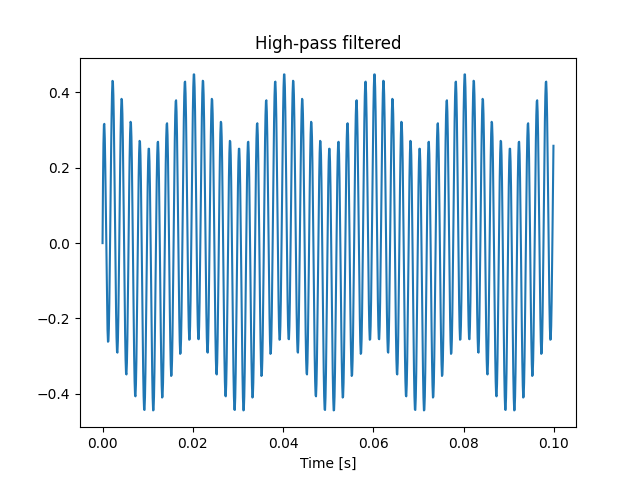
\includegraphics[width=0.45\linewidth]{results/figures/task4_8_highpass_filtered.png}
\hfill
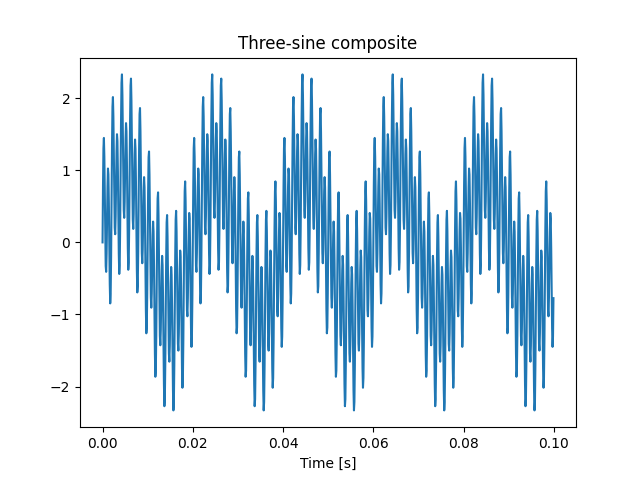
\includegraphics[width=0.45\linewidth]{results/figures/task4_9_sum_three_sine_waves.png}

\medskip
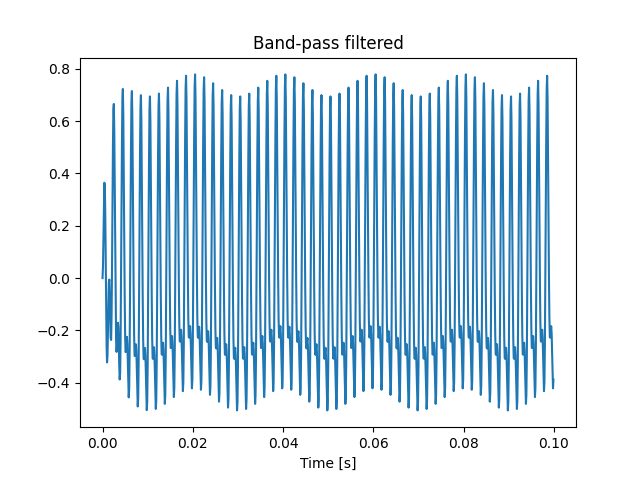
\includegraphics[width=0.45\linewidth]{results/figures/task4_12_bandpass_filtered.png}
\caption{Filtering outputs for Task 4.}
\end{figure}
%---------------------------------------------------------------
\subsection*{R.4.1 Detail the design process of the filter in T.4.3. Draw the required circuit and calculate the value for the components step by step.}

A first–order passive low-pass was built with a series resistor and a shunt capacitor.  
Selecting the default value used in the code (\texttt{rc\_lowpass(50)}), $R$ is fixed to $1\,\mathrm{k}\Omega$ and  
\[
C=\frac{1}{2\pi f_c R}=\frac{1}{2\pi\,(50)\,(1\,000)}\approx 3.18\,\mu\mathrm{F}.
\]
The −3 dB corner frequency is verified by $f_c = 1/(2\pi RC)$.  
The circuit is: input → $R$ → node; node → $C$ → ground; node is the output.

%---------------------------------------------------------------
\subsection*{R.4.2 Detail the design process of the filter in T.4.4. Derive the equation to implement the filter step by step on a data stream.}

In the script a 1-st-order digital Butterworth low-pass is generated by  
\texttt{butter\_lowpass(50, fs=10\,000, order=1)}.  
The bilinear transform maps the analog prototype \( H(s)=\frac{\omega_c}{s+\omega_c} \) to  
\( H(z)=\frac{b_0+b_1z^{-1}}{1+a_1z^{-1}} \).  
Scipy returns
\[ y[n]=b_0\,x[n]+b_1\,x[n-1]-a_1\,y[n-1]. \]
With \(f_s=10\,000\) Hz and \(f_c=50\) Hz the coefficients are
\( b_0=b_1\approx0.0155,\; a_1\approx-0.969 \) (see \texttt{b,a} in the code).
This equation is applied sample-by-sample using \texttt{scipy.signal.lfilter}.

%---------------------------------------------------------------
\subsection*{R.4.3 Detail the design process of the filter in T.4.6. Draw the required circuit and calculate the value for the components step by step.}

For a passive high-pass the positions of $R$ and $C$ are swapped.  
Using \texttt{rc\_highpass(500)} the script again fixes $R=1\,\mathrm{k}\Omega$:  
\[
C=\frac{1}{2\pi f_c R}=\frac{1}{2\pi\,(500)\,(1\,000)}\approx 0.32\,\mu\mathrm{F}.
\]
Circuit: input → $C$ → node; node → $R$ → ground; node is the output.

%---------------------------------------------------------------
\subsection*{R.4.4 Detail the design process of the filter in T.4.7. Derive the equation to implement the filter step by step on a data stream.}

\texttt{butter\_highpass(500, fs=10\,000, order=1)} gives
\( H(z)=\frac{b_0+b_1z^{-1}}{1+a_1z^{-1}} \) with
\( b_0\approx0.863,\; b_1\approx-0.863,\; a_1\approx-0.727. \)
The resulting difference equation is  
\( y[n]=b_0\,x[n]+b_1\,x[n-1]-a_1\,y[n-1]. \)

%---------------------------------------------------------------
\subsection*{R.4.5 Detail the design process of the filter in T.4.10. Draw the required circuit and calculate the value for the components step by step.}

An active band-pass is formed by cascading a high-pass and a low-pass stage around an op-amp buffer.
Calling \texttt{rc\_bandpass(400,600)} selects the default $R=1\,\mathrm{k}\Omega$ and computes
\[
C=\frac{1}{2\pi\,(600)\,(1\,000)}\approx0.27\,\mu\mathrm{F}.
\]
Both RC sections use this $R$ and $C$, giving a pass band centred near $500\,$Hz. The op-amp prevents interaction between stages and can provide gain.

%---------------------------------------------------------------
\subsection*{R.4.6 Detail the design process of the filter in T.4.11. Derive the equation to implement the filter step by step on a data stream.}

The digital band-pass is produced in one call:
\texttt{butter\_bandpass(400,600, fs=10\,000, order=1)}.  
Internally this designs a Butterworth HP and LP, combines them, and yields
\( H(z)=\frac{b_0+b_1z^{-1}+b_2z^{-2}}{1+a_1z^{-1}+a_2z^{-2}} \)  
with coefficients automatically calculated by Scipy.  
The sample stream is filtered with \texttt{lfilter(b, a, data)}.

%---------------------------------------------------------------
\subsection*{R.4.7 What is the difference between passive and active filters?}

Passive filters use only $R$, $L$, $C$ and cannot amplify; active filters add powered devices (op-amps, transistors) so they can buffer, amplify, and avoid large inductors.

%---------------------------------------------------------------
\subsection*{R.4.8 What is the difference between FIR and IIR filters?}

FIR filters have a finite impulse response and are always stable; IIR filters have feedback, achieve sharper roll-off with fewer coefficients, but can become unstable and introduce nonlinear phase.

%---------------------------------------------------------------
\subsection*{R.4.9 What is the “order” of a discrete filter?}

Order equals the highest delay term $z^{-k}$ (number of poles).  It determines the slope: each order adds about 20 dB/decade attenuation.

%---------------------------------------------------------------
\subsection*{R.4.10 How could you implement a continuous-time filter in a robotic system?}

Place an analog RC/active filter between the sensor output and the ADC to pre-condition the signal before sampling.

%---------------------------------------------------------------
\subsection*{R.4.11 How could you implement a discrete-time filter in a robotic system?}

Run the filter’s difference equation in firmware (MCU/DSP) at the sampling rate, using fixed-point or floating-point arithmetic.

%---------------------------------------------------------------
\subsection*{R.4.12 What are the advantages and disadvantages of analog and digital filters in robotic systems?}

Analog: zero latency, no quantisation, low power; but component drift, no re-tuning in software.  
Digital: reconfigurable, repeatable, high order; but needs ADC/DAC, adds latency and quantisation noise.

%---------------------------------------------------------------
\subsection*{R.4.13 Is it possible to make a 1000 Hz Low-Pass filter in a digital system with a sampling rate of 1000 Hz?}

No.  The Nyquist limit is 500 Hz, so a 1000 Hz cut-off is unattainable without a higher sampling rate.

%---------------------------------------------------------------
\subsection*{R.4.14 Deliver the code to generate the signals and the plots (T.4.1 – T.4.12).}

All figures were produced by \texttt{scripts/task4\_filtering.py}, which calls
\texttt{src/filter\_design.py} and \texttt{src/signal\_generation.py}.  
Key lines:

\begin{verbatim}
# signal generation
fs = 10000
t, signal = sum_sine_waves([(50,1.0),(500,0.5)], fs, 0.1)

# low-pass
b_lp, a_lp = butter_lowpass(50, fs, order=1)
filtered_lp = apply_filter(signal, b_lp, a_lp)

# high-pass
b_hp, a_hp = butter_highpass(500, fs, order=1)
filtered_hp = apply_filter(signal, b_hp, a_hp)

# band-pass
b_bp, a_bp = butter_bandpass(400, 600, fs, order=1)
filtered_bp = apply_filter(signal + 
    sum_sine_waves([(1000,1.0)], fs, 0.1)[1], b_bp, a_bp)
\end{verbatim}



%--------------------------------------------------------------------
\end{document}
